\documentclass{pssbmac}

%%%%%%%%%%%%%%%%%%%%%%%%%%%%%%%%%%%%%%%%%%%%%%%%%%%%%%%%%%%%%%%%%%%%%%%%
%% POR FAVOR, NÃO FAÇA MUDANÇAS NESSE PADRÃO QUE ACARRETEM  EM
%% ALTERAÇÃO NA FORMATAÇÃO FINAL DO TEXTO
%%%%%%%%%%%%%%%%%%%%%%%%%%%%%%%%%%%%%%%%%%%%%%%%%%%%%%%%%%%%%%%%%%%%%%%%

%%%%%%%%%%%%%%%%%%%%%%%%%%%%%%%%%%%%%%%%%%%%%%%%%%%%%%%%%%%%%%%%%%%%%%%%
% POR FAVOR, ESCOLHA CONFORME O CASO
%%%%%%%%%%%%%%%%%%%%%%%%%%%%%%%%%%%%%%%%%%%%%%%%%%%%%%%%%%%%%%%%%%%%%%%%
\usepackage[brazil]{babel} % texto em Português
%\usepackage[english]{babel} % texto em Inglês

%\usepackage[latin1]{inputenc} % acentuação em Português ISO-8859-1
\usepackage[utf8]{inputenc} % acentuação em Português UTF-8
%%%%%%%%%%%%%%%%%%%%%%%%%%%%%%%%%%%%%%%%%%%%%%%%%%%%%%%%%%%%%%%%%%%%%%%%


%%%%%%%%%%%%%%%%%%%%%%%%%%%%%%%%%%%%%%%%%%%%%%%%%%%%%%%%%%%%%%%%%%%%%%%%
%% POR FAVOR, NÃO ALTERAR
%%%%%%%%%%%%%%%%%%%%%%%%%%%%%%%%%%%%%%%%%%%%%%%%%%%%%%%%%%%%%%%%%%%%%%%%
\usepackage[T1]{fontenc}
\usepackage{float}
\usepackage{graphics}
\usepackage{graphicx}
\usepackage{epsfig}
\usepackage{indentfirst}
\usepackage{amsmath, amsfonts, amssymb, amsthm}
\usepackage{url}
\usepackage{csquotes}
% Ambientes pré-definidos
\newtheorem{theorem}{Theorem}[section]
\newtheorem{lemma}{Lemma}[section]
\newtheorem{proposition}{Proposition}[section]
\newtheorem{definition}{Definition}[section]
\newtheorem{remark}{Remark}[section]
\newtheorem{corollary}{Corollary}[section]
\newtheorem{teorema}{Teorema}[section]
\newtheorem{lema}{Lema}[section]
\newtheorem{prop}{Proposi\c{c}\~ao}[section]
\newtheorem{defi}{Defini\c{c}\~ao}[section]
\newtheorem{obs}{Observa\c{c}\~ao}[section]
\newtheorem{cor}{Corol\'ario}[section]

% ref bibliográficas
\usepackage[backend=biber, style=numeric-comp, maxnames=50]{biblatex}
\addbibresource{refs.bib}
\DeclareTextFontCommand{\emph}{\boldmath\bfseries}
\DefineBibliographyStrings{brazil}{phdthesis = {Tese de doutorado}}
\DefineBibliographyStrings{brazil}{mathesis = {Disserta\c{c}\~{a}o de mestrado}}
\DefineBibliographyStrings{english}{mathesis = {Master dissertation}}
%%%%%%%%%%%%%%%%%%%%%%%%%%%%%%%%%%%%%%%%%%%%%%%%%%%%%%%%%%%%%%%%%%%%%%%%


\DeclareMathOperator{\diag}{diag}
\begin{document}

%%%%%%%%%%%%%%%%%%%%%%%%%%%%%%%%%%%%%%%%%%%%%%%%%%%%%%%%%%%%%%%%%%%%%%%%
% TÍTULO E AUTORAS(ES)
%%%%%%%%%%%%%%%%%%%%%%%%%%%%%%%%%%%%%%%%%%%%%%%%%%%%%%%%%%%%%%%%%%%%%%%%

\title{Otimização de Geometria Molecular}

\author{
    {\large Felipe Fernandes G. S. Costa}\thanks{fernandes.felipe@aluno.ufabc.edu.br} \\
    {\small BC\&T/UFABC, Santo André, SP} \\
    {\large Yuri Alexandre Aoto}\thanks{yuri.aoto@ufabc.edu.br} \\
    {\small CMCC/UFABC, Santo André, SP} \\
}
\criartitulo
%%%%%%%%%%%%%%%%%%%%%%%%%%%%%%%%%%%%%%%%%%%%%%%%%%%%%%%%%%%%%%%%%%%%%%%%


%%%%%%%%%%%%%%%%%%%%%%%%%%%%%%%%%%%%%%%%%%%%%%%%%%%%%%%%%%%%%%%%%%%%%%%%
% TEXTO
%%%%%%%%%%%%%%%%%%%%%%%%%%%%%%%%%%%%%%%%%%%%%%%%%%%%%%%%%%%%%%%%%%%%%%%%

Na área da química computacional, um de seus tópicos de interesse é a otimização de geometrias moleculares de reações químicas com uso de métodos iterativos. As funções de Superfície de Energia Potencial (SEP) descrevem qual a energia associada a uma configuração de moléculas, configurações essas representadas pelas distâncias de ligações dos átomos e suas angulações. Essas funções podem ser descritas no formato $F: U \subset R^k\to R$ com $k \in N$, por conta disso é comumente utilizado o método de Newton para a otimização dessas funções, ou seja, para localização de mínimos locais, que nesse contexto, podem representar a configuração ótima de uma molécula em um estado estacionário de uma reação química.

O método de Newton tende a apresentar resultados satisfatórios de convergência. Para casos suficientemente próximos dos pontos críticos a sua convergência é quadrática, e existem teoremas \cite{calculo_numerico_aplicado} que garantem a sua convergência em uma determinada vizinhança do ponto crítico. Contudo, o método possui um custo computacional considerável, isso porque para cada etapa de iteração é necessário calcular $k^2$ derivadas segundas e inverter uma matriz $k \times k$. Pelo fato de funções SEP usualmente não possuírem expressões analíticas, o cálculo de suas derivadas é feito numericamente, tornando-o custoso principalmente para funções que exigem alto tempo computacional.

O objetivo desse trabalho é desenvolver um método, baseando-se no método de Newton, que reduza o custo computacional de cada etapa de iteração, permanecendo com uma taxa de convergência similar ao método de Newton para problemas de otimização da química computacional. Para isso, será utilizado como função SEP \cite{fh2o_sep_fortran_module} de otimização a reação $F + H_2O \to FH + HO$. Essa reação possui 5 pontos estacionários com geometrias ótimas e valores de energia associados conhecidos \cite{fh2o_first_sep}. Dessa maneira, o método desenvolvido denominado CBPD (\textit{Convergence Based in Partials Derivatives}), será validado otimizando geometrias próximas de ponto estacionário da reação.

Seja $x_n \in R^k$ referente ao enésimo ponto do processo de otimização. Utilizando o método de Newton, um novo ponto $x_{n+1}$ é definido calculando
%
\begin{equation}
  x_{n+1} = x_n - H_F(x_n)^{-1} \nabla F(x_n) \,,
\end{equation}
%
sendo $H_F(x_n)^{-1}$ a matriz inversa $k \times k$ da hessiana da função $F$ e $\nabla F$ o vetor gradiente da função $F$.
No método CBPD, que se baseia em considerar cada derivada parcial um caso isolado de otimização, um novo ponto $x_{n+1}$ é definido calculando
%
\begin{equation}
  x_{n+1} = x_n - \diag{\left(\frac{\partial^2 F}{\partial (x_{n})^2 }\right)}^{-1} \nabla F(x_n) \,,
\end{equation}
%
sendo diag a matriz diagonal da matriz hessiana da função $F$.

O método CBPD por utilizar apenas a diagonal da matriz hessiana, implica que para cada etapa de iteração seja necessário calcular $k$ derivadas segundas e não é necessário inverter a matriz. Além disso, para diminuir o custo computacional do cálculo das derivadas parciais é utilizado uma aproximação do valor das derivadas baseado no método da Secante, que de acordo com o Teorema de Valor Médio \cite{calculo_1} afirma que existe uma reta tangente com inclinação exatamente igual à da reta secante descrita por dois pontos de uma função caso a função seja diferenciável.

Em termos de resultados, utilizando a função PES de estudo e criando cenários para convergência dos quais apenas uma coordenada de cada vez era alterada com taxas de variação de até 25\% do valor ótimo da configuração do ponto estacionário, foram calculadas as taxas de sucesso de convergência tanto para o método CBPD, quanto para o método de Newton como apresentados na Figura \ref{figura01}.
%
\begin{figure}[H]
\centering
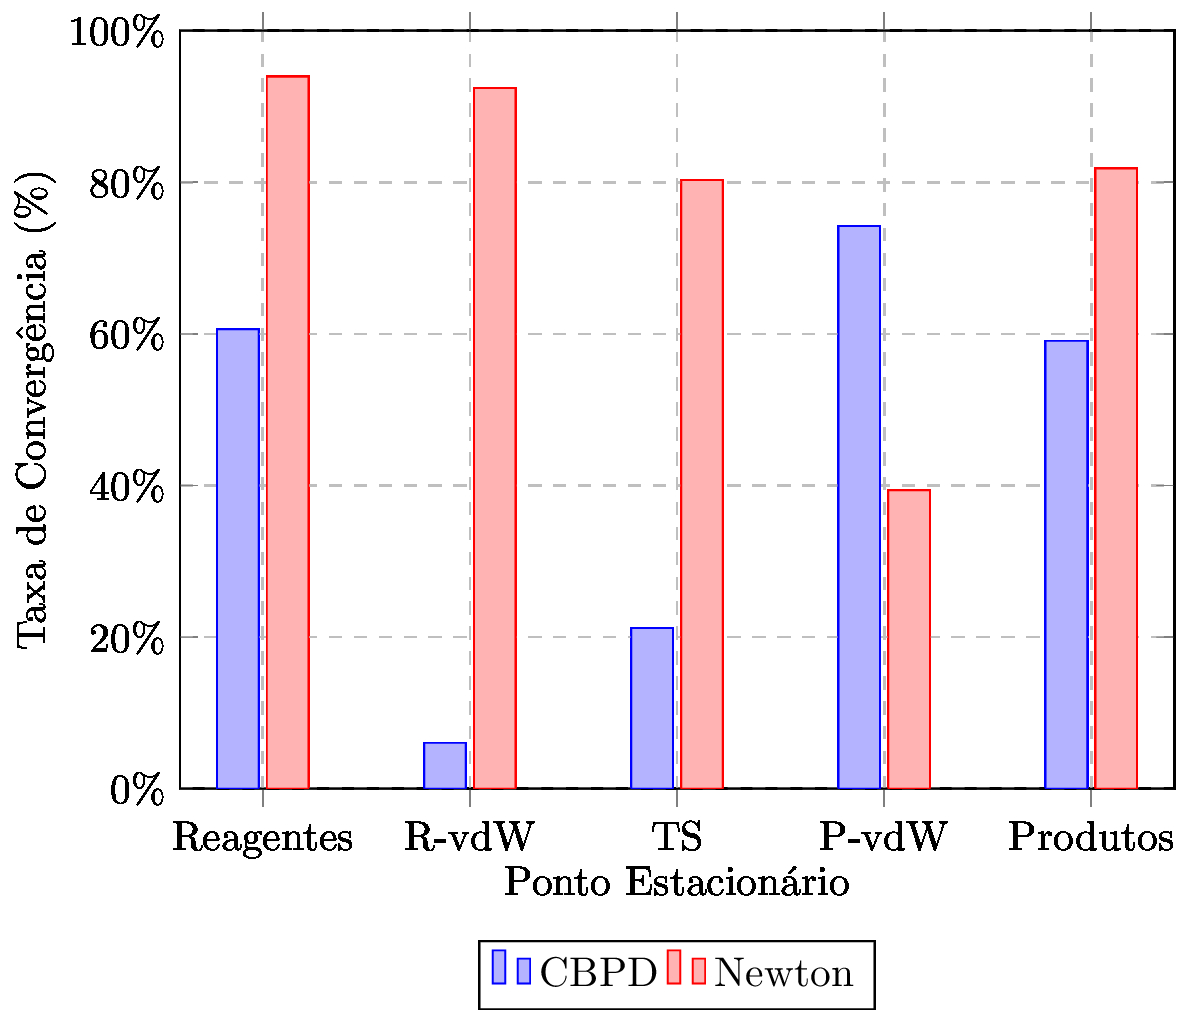
\includegraphics[width=.425\textwidth]{image}
\caption{ {\small Gráfico de taxa de convergência do método CBPD em comparação com método de Newton com casos de variação de uma coordenada das configurações ótimas para cada ponto estacionário da reação. Fonte: autoria própria.}}
\label{figura01}
\end{figure}
%
Apesar do método CBPD apresentar um resultado inferior em taxa de convergência quando comparado com o método de Newton para a maioria dos pontos estacionários, alguns pontos estacionários possuem um sucesso de convergência satisfatório e equiparável ao método de Newton, que possui um maior custo computacional relacionado. Diante disso, a depender dos cenários de convergência, o método CBPD pode ser uma alternativa para realizar o processo de otimização com um menor custo computacional.

%%%%%%%%%%%%%%%%%%%%%%%%%%%%%%%%%%%%%%%%%%%%%%%%%%%%%%%%%%%%%%%%%%%%%%%%
% REFS BIBLIOGRÁFICAS
% POR FAVOR, NÃO ALTERAR
%%%%%%%%%%%%%%%%%%%%%%%%%%%%%%%%%%%%%%%%%%%%%%%%%%%%%%%%%%%%%%%%%%%%%%%%
\printbibliography
%%%%%%%%%%%%%%%%%%%%%%%%%%%%%%%%%%%%%%%%%%%%%%%%%%%%%%%%%%%%%%%%%%%%%%%%

\end{document}




